\section{Dawson's Chess on the Cylinder}\label{sec:dawson}

On a cylinder every file is alike, and the first move opens the ring of files into an ordinary strip. The
earlier study~\cite{Study2025} used this idea on Dawson's chess but stated the game incorrectly; we
redo it.



\emph{Rules.} Dawson's chess~\cite{Dawson1935} is played on a $3\times n$ board
(Section~S9 shows the boards) with white pawns on rank~1, black pawns on rank~3 and rank~2 empty. Pawns move
and capture as in chess, captures are compulsory, and no pawn can double-step or promote. The last player to
move wins; in the mis\`ere form that Dawson posed, the last player loses.

Call a file \emph{untouched} if both its pawns stand on their starting squares. If white plays c1--c2 with the
b- and d-files untouched, the captures b3$\times$c2, d1$\times$c2, d3$\times$c2 and b1$\times$c2 are forced
(up to the choice of side), and leave black to move with the b- and d-files empty and the c-file blocked for
good. At the end of a row the push takes three plies and empties its one neighbor; a push with no untouched
neighbor is blocked. Counting each forced sequence as one move, strips separated by empty files never interact,
and the game is impartial: a strip of $n$ untouched files is the octal game
$\mathbf{0.137}$~\cite{GuySmith1956,WinningWays}, in which a move removes a file and its untouched neighbors. Its
Grundy values are $g(0)=0$, $g(1)=1$ and, for $n\ge2$,
\begin{equation}\label{eq:dawson}
g(n)=\operatorname{mex}\bigl(\{g(n-2)\}\cup\{g(a)\oplus g(b) : a+b=n-3\}\bigr),
\end{equation}
where $a,b\ge0$, $\oplus$ is the nim-sum and mex the least non-negative integer not in the set. The first
player wins the ordinary $3\times n$ board exactly when $g(n)\ne0$. The values have period 34 with last exception
$n=51$~\cite{GuySmith1956}, which two programs reproduce for $n\le300$ \lab{C2}.

\emph{What was wrong.} In~\cite{Study2025} a pawn could be removed from a single row only when both its
neighbors were empty, so a full row of two or more pawns has no move. Its recurrence lacks the end-file term
$g(n-2)$ and the value $g(1)=1$, agrees with $g$ at only 31 of the 301 values $n\le300$, and gives the wrong
cylinder outcome for 56 of them, the first at $n=4$ \lab{C2}.

\begin{theorem}[Ring rule; \lab{P}, machine-checked for $n\le16$]\label{thm:ring}
On the full $3\times n$ cylinder, $n\ge3$, every first move with its forced captures leaves one strip of
$n-3$ untouched files, with the opponent to move. Hence the cylinder has Grundy value
$\operatorname{mex}\{g(n-3)\}$, and the first player wins if and only if $g(n-3)=0$, that is, for
$n=3,7,11,17,23,27,31,37,41,45,57,\dots$
\end{theorem}

\begin{proof}
Every file of a full ring has two distinct untouched neighbors, so every push starts the five-ply sequence
above. The other $n-3$ files, bounded by empty files that never change, form an ordinary strip. By
rotation all first moves are alike, and the cylinder has one option.
\end{proof}

\begin{figure}[!t]
\centering
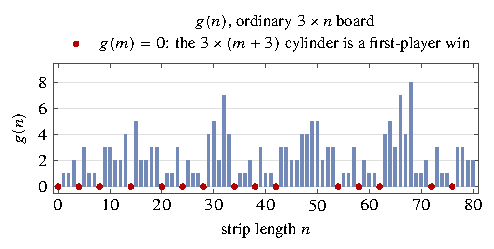
\includegraphics{figures/dawson_grundy.pdf}
\caption{Grundy values $g(n)$ of Dawson's chess on the $3\times n$ ordinary board (octal game
$\mathbf{0.137}$), $n\le80$. Dots mark $g(m)=0$: the $3\times m$ board is a second-player win and the
$3\times(m+3)$ cylinder a first-player win (Theorem~\ref{thm:ring}).}
\label{fig:dawson_grundy}
\end{figure}

The ring formula of~\cite{Study2025}, and its remark that the ring's value is 0 or 1, hold with the correct $g$
(Fig.~\ref{fig:dawson_grundy}). In mis\`ere play the ring rule carries over, since a forced sequence has odd
length (the first player wins exactly when the $(n-3)$-file strip is a mis\`ere P-position); our implementation of the Plambeck--Siegel algorithm~\cite{PlambeckSiegel2008} reproduces their partial
quotient for strips of at most 32 files (order 638, 109 P-positions) \lab{C2}, and the next quotient did not
finish (Section~S9).
